\begin{figure}%[tbp]
	\begin{subfigure}[b]{.23\textwidth}
	\centering
	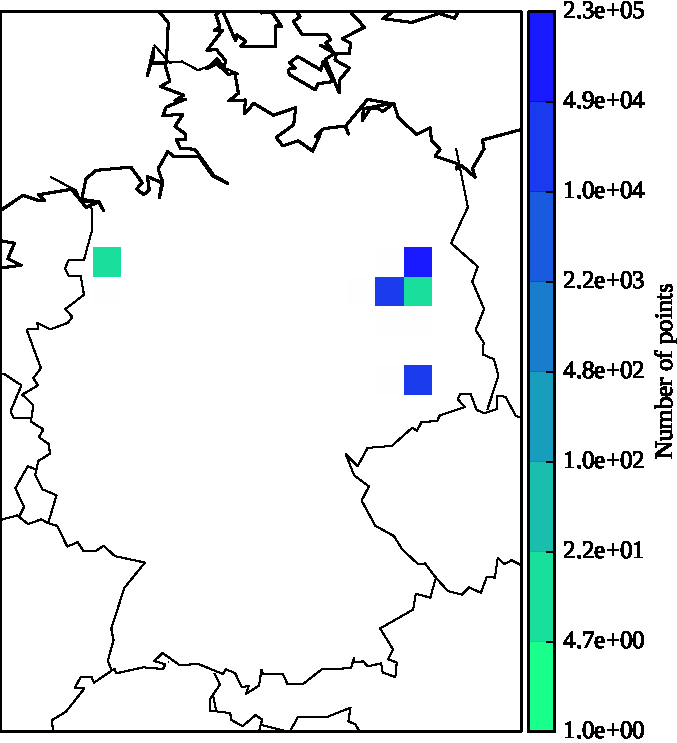
\includegraphics[width=\textwidth]{pix/freq_COM_ger_berlin.pdf}
		\caption{CM}
		%\label{fig:gull}
	\end{subfigure}
	%\,
	\begin{subfigure}[b]{.23\textwidth}
	\centering
	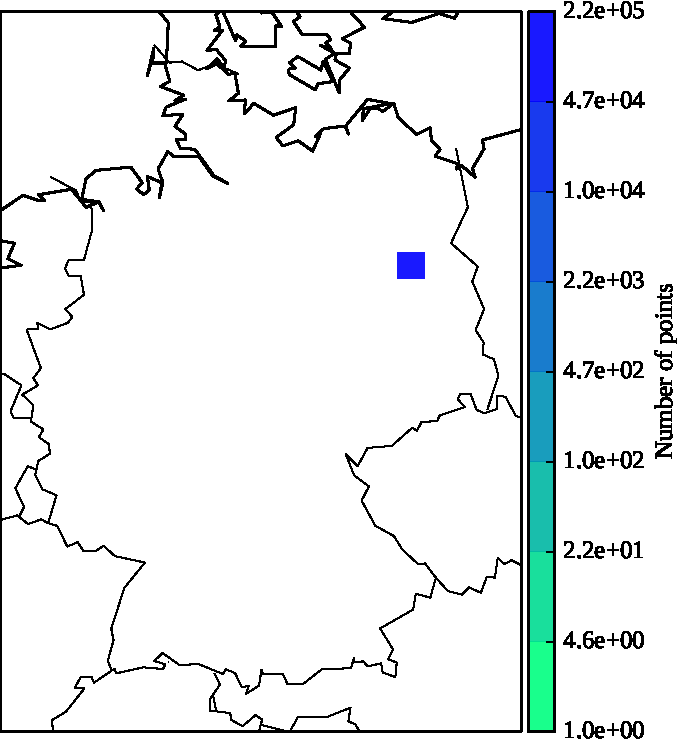
\includegraphics[width=\textwidth]{pix/freq_RW_ger_berlin.pdf}
		\caption{GM}
		%\label{fig:gull}
	\end{subfigure}
	\hfill
	\begin{subfigure}[b]{.23\textwidth}
	\centering
	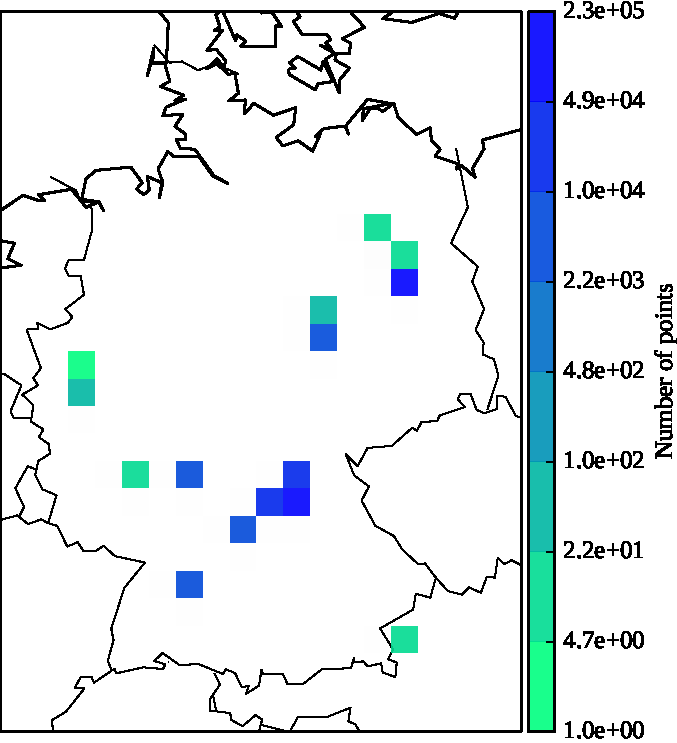
\includegraphics[width=\textwidth]{pix/freq_COM_ger_oster.pdf}
		\caption{CM}
		%\label{fig:gull}
	\end{subfigure}
	%\,
	\begin{subfigure}[b]{.23\textwidth}
	\centering
	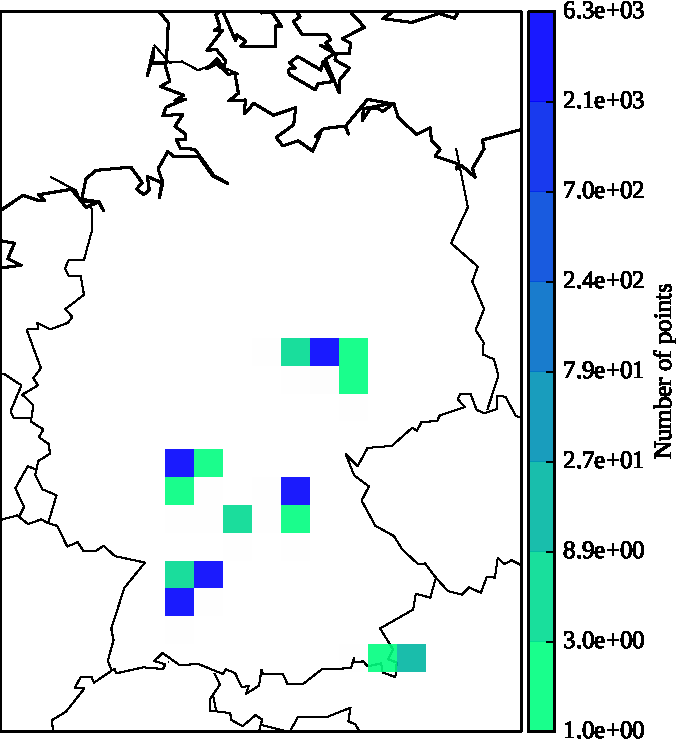
\includegraphics[width=\textwidth]{pix/freq_RW_ger_oster.pdf}
		\caption{GM}
		%\label{fig:gull}
	\end{subfigure}
	%
	\caption[Distributions for \emph{berlin}, \emph{oster} using dataset B.]{The left two distributions show $CM$ and $GM$ for \emph{berlin}, while the right pictures visualise the term \emph{oster} for dataset B.}
	\label{fig:B_comp}
\end{figure}